\chapter{Design}
\label{design}

% The design should describe what you expected to do, and might also explain areas that you had to revise after some investigation.

% Typically, for an object-oriented design, the discussion will focus on the choice of objects and classes and the allocation of methods to classes. The use made of reusable components should be described and their source referenced. Particularly important decisions concerning data structures usually affect the architecture of a system and so should be described here.

% How much material you include on detailed design and implementation will depend very much on the nature of the project. It should not be padded out. Think about the significant aspects of your system. For example, describe the design of the user interface if it is a critical aspect of your system, or provide detail about methods and data structures that are not trivial. Do not spend time on long lists of trivial items and repetitive descriptions. If in doubt about what is appropriate, speak to your supervisor.

% You should concentrate on the more important aspects of the design. It is essential that an overview is presented before going into detail. As well as describing the design adopted it must also explain what other designs were considered and why they were rejected.

\section{Introduction}
The technical design of an application is, in essence, the intersection of current ``best practice'' in the software development field (and the related programming language communities), its target domains and the user needs.

``Technically'', FundFind:
\begin{itemize}
 \item is a web application
 \item is written in Python
 \item stores its data in an asynchronous NoSQL data store with built-in search capabilities
 \item has a mobile-friendly web interface
 \item exposes all its major features via an API
\end{itemize}

These characteristics have not changed since the start of the project. The technical decisions that stand behind them proved to be mostly correct and helpful, and are elaborated upon in the next section.

The parent IDFind project had not done anything like one of the new features which were added during development - harvesting funding data from machine-readable sources. The new Funding Harvest feature is actually technically separate from the rest of FundFind's codebase - it just puts whatever information it finds in FundFind's datastore and the only link between the two codebases is the datastore. Developing it separately made sense as it can thus be readily re-used and changed.

\subsection{Design Details and Rationale}
\label{design-rationale}

FundFind
\begin{itemize}
 \item is a web application
 
This was decided right from the start of the project. The way current Open Knowledge Foundation and Cottage Labs projects worked was important since one of the two major target domains is Open Data / Knowledge and Cottage Labs is an interested party. Most OKFN projects are web applications - even the library ones have mostly been used in web applications. Cottage Labs have also focussed on web applications. Such applications have just proven themselves to be far more ``co-operative'' than traditional desktop applications - easy to access, easy to modify so that they expose their data via an API (interoperability). \S\ref{api-tech-design} details further interoperability decisions - the transport format (JSON) and protocol (HTTP).
 
 \item is written in Python

Similar factors to the interoperability point raised above played a role in deciding the language of the application. A lot of Open Knowledge projects use Python \cite{nomenklatura, offenesparlament, pybossa, activityapi} - the same goes for Cottage Labs projects \cite{leaps, portality, iioa, artemis, cl-web-code, xcri, negotiator}. The language is also simple and strives encourage and enable readability - ``code is read much more often than it is written'' \cite{pep8}.
 
 \item stores its data in an asynchronous NoSQL data store with built-in search capabilities
 
 FundFind relies on elasticsearch to store its data. Elasticsearch is an indexing server which allows for sophisticated search queries against a body of text and other data \cite{es}. The essential advantages were simplicity, performance, usage by other Cottage Labs projects and certain options it leaves open for further development (see \S\ref{design-datastore}).
 
 \item has a mobile-friendly web interface
 
 FundFind is an application which tries to enable sharing of information - one of the highest priority features. Owing to the nature of the information it makes sense to try to make it mobile-friendly - scholars do not necessarily have to hear about funding opportunities while sitting at their desks.
 
 Whether they will also want to share this rather dense information while on the go is another matter entirely. Mobile-friendliness was not noted as having particularly high priority in the Progress Report, and it still does not - it was just easy to implement due to the fact that the libraries used to make the web user interface follow current best software engineering practice. More details are available in \S\ref{impl-ui}. Essentially, making a good UI by using the libraries properly would have led to a mobile-friendly UI (at the flick of a filename and a few CSS class names).
 
 \item exposes all its major features via an API
 
 The JISC Report ``Advantages of APIs'' states ``the API enables use and re-use; it is a tool by which we can disseminate knowledge'' \cite{advantages-apis}. This is the essential advantage of API-s and the reason the concept of an API has become one of the building blocks of the Open Knowledge movement. If FundFind aims to prototype a useful tool which will eventually contribute to Open Data (so taking into account the needs of the ``analytical'' audience group from \S\ref{audience-analyse}), it needs to eventually have an API. It is simply better to design the project with the API in mind instead of tacking it on later. One example is the HiFi project, which had the following to say on the subject:
 
 \begin{shadequote}
  We built the API to satisfy these requirements first, then we built our app on top of the API. This turned out to be a great idea. We got to dogfood our API for the entire development process and it made testing a lot simpler.
  \par\emph{Kris Jordan in ``First we built an API, then we built a CMS'' \cite{hifi-api}}
 \end{shadequote}
 
\end{itemize}

\section{Overall Architecture}
% diagram of architecture
% changes from progress report - any?, why? why not?
% these are all MODULES, not CLASSES - explain difference, rationale for using (convention at least)

\begin{figure}[H]
\centering
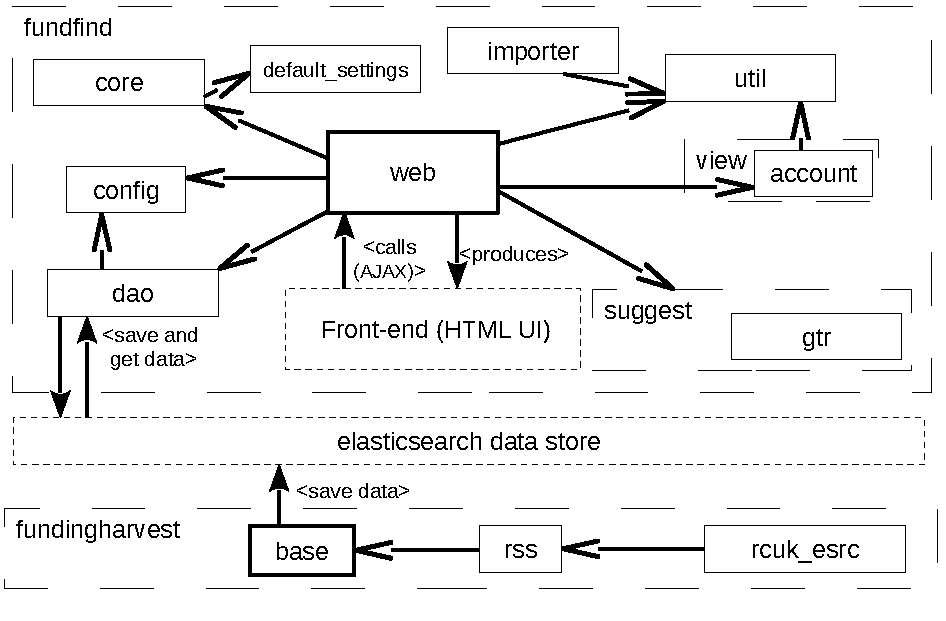
\includegraphics[width=1.00\textwidth,]{Chapter3/overview_design.pdf}
\caption{Overview of FundFind and Funding Harvest's technical architecture.}
\label{fig:arch}
\end{figure}

The entities drawn with continuous lines in the diagram are modules - collections of code related to solving the same problem. The contents of the modules - the details of the technical design of the main application - are discussed below in \S\ref{design-main-first} to \S\ref{design-main-last}.

The entities drawn with a heavy continuous line are the entry points - they are the modules which actually (need to) get run by the Python interpreter.

The entities drawn with a rough dashed line are packages. Packages and modules are simply ways of organising code in Python and are discussed in more detail below.

The entities drawn with a fine dashed line are more abstract concepts (datastore and user interface) which are elaborated upon below.

Full listing of all source code files with notes is available in ``\titleref{file-listings}'', Appendix \ref{file-listings}.

\subsection{Organising code in Python}
Traditionally Object-Oriented Programming talks about ``classes'' as, essentially, blueprints combining data structures and imperative code (methods) together. These can then be ``instantiated'' to produce a concrete ``object''.

This is of course well-supported in Python. However, Python also has an additional convention when it comes to organising code - ``modules''. The Python documentation says ``You may also want to use a handy function that you’ve written in several programs without copying its definition into each program.'' \cite{python-doc-modules}. While re-use of code is usually achieved by making everything an object in other languages like Java, Python actually allows functions and even just code statements at the top level of a source code file. Thus, instead of having to create a ``Util'' class with several static methods, Python authors are encouraged to simply define the functions they need at the module level. In other words, modules are a convenient way to bundle together \emph{related} pieces of code - whether that would just be a sequence of statements, function or class definitions. This may seem messy but has proven to be quite efficient by essentially allowing the developer to better express their mental model 
of how their program should be organised, instead of forcing a particular structure.

An obvious characteristic of Python modules is that they are also implicit namespaces. Thus, the built-in |int()| can easily be distinguished from |random.int()|. A Python program would have to |import random| before it can use |random.int()|.

In this case, |random| happens to be a module that is part of the standard Python distribution. However, exactly the same rules apply to user-defined modules. Thus, the |<uses>| arrows which connect the modules in Figure \ref{fig:arch} essentially mean ``module X imports module Y and uses something from Y''.

Packages are simply a collection of modules. Since a module is a file, packages are just directories (containing a possibly empty |__init__.py| file) - another way to organise related code.

To sum up, packages contain modules. Modules could contain classes (alongside any other code and function definitions).

Furthermore, certain naming conventions exist in Python for package, module and class names, which account for the names used in fundfind and fundingharvest projects.

\begin{shadequote}
Modules should have short, all-lowercase names. Underscores can be used in the module name if it improves readability. Python packages should also have short, all-lowercase names, although the use of underscores is discouraged.

[...]

Almost without exception, class names use the CapWords convention.

Style Guide for Python Code, Prescriptive: Naming Conventions \cite{pep8}
\end{shadequote}

\subsection{Changes over time}
\label{design-changes}
% TODO redo this with a diagram showing the real initial IDFind code and showing deleted modules in red, added modules in green
The core modules which form the main web application have not changed much from the parent IDFind project. The diagram of IDFind's technical design presented in the Progress Report \cite{progress-report} was meant to be an overview diagram and had left out several details. These are presented in Figure \ref{fig:idfind-new-uml}.

Some of the modules which have been deleted during FundFind's development merit further discussion:
\begin{itemize}
	\item |tweetlisten| allows IDFind to respond to Twitter requests in a similar fashion as if the user was using the web user interface.
	
	This module was scrapped in FundFind since potential target users (including the author) just could not think of a way in which Twitter integration would be \emph{immediately} useful. There was also an issue with the inherited tests, discussed in \myref{testing-intro}.
%TODO describe other changes as per diagram
\end{itemize}

In terms of changes, the contents of all of these modules have of course changed to accommodate FundFind's aims.

%TODO include different diagram here
\begin{figure}[H]
\centering
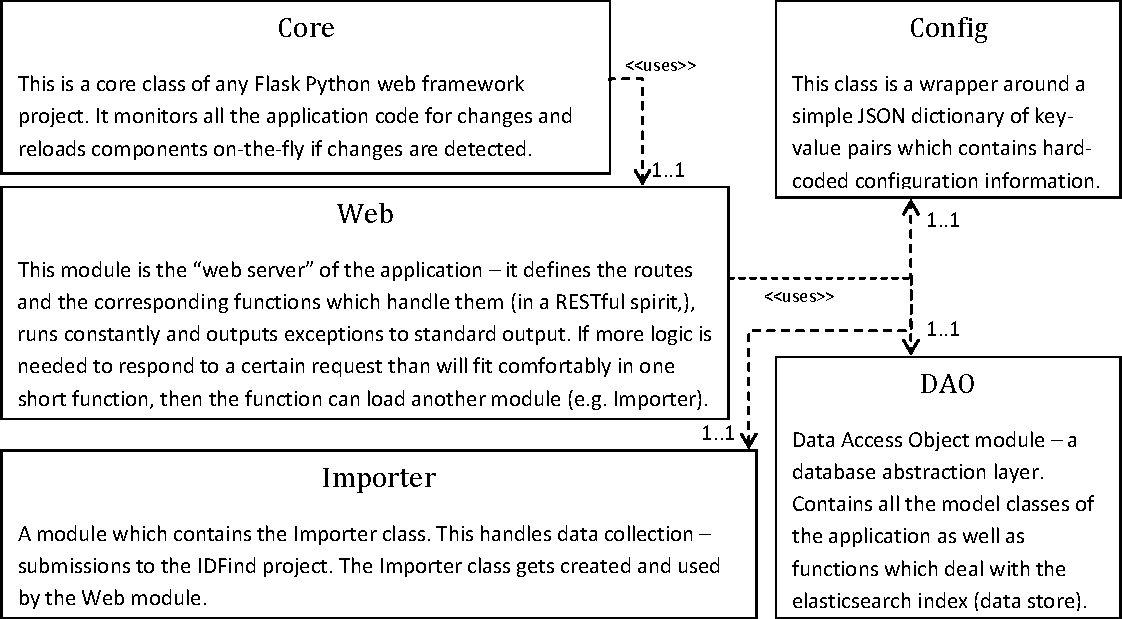
\includegraphics[width=1.00\textwidth,]{Chapter3/idfind-uml.pdf}
\caption{Overview of parent project IDFind's technical design presented in the Progress Report \cite{progress-report}. This should include several more modules, coloured in red (deleted for FundFind) and black (left in).}
\label{fig:idfind-new-uml}
\end{figure}

\section{Datastore}
\label{design-datastore}
A discussion of the nature of the slightly unconventional datastore is in order since it has informed the technical design of both FundFind and Funding Harvest.

 Indexing software is usually most easily understood in comparison to more traditional approaches of storing data, like relational databases (MySQL \cite{mysql}, Oracle \cite{oracle}). These store data in a highly structured way and the base structural unit is a table (theoretically equivalent to a set, which is where relational theory and such databases come from). The ``indexing'' part actually means ``analysis'' in the broadest sense. Given data - any data, images, text, Microsoft Word binary blobs pretending to be text - the software will try to find common features or look for certain characteristics in the data. For example, it will try to discern whether a particular string actually represent a datetime value.
 
 Elasticsearch is actually a NoSQL datastore - which essentially means that it deals with very simple key-value pairs as the basic unit of organising data \emph{instead of} tables, or sets. It also supports slightly more complex, but still very simple structures, such as lists and dictionaries (a.k.a. HashMaps). This means that the storage representation is also quite simple - in this case, all documents stored within an elasticsearch instance can be represented in the JSON data format. This simplicity enables elasticsearch to deal with semistructured data much more easily than a traditional relational database.
 
 In terms of individual values, it should be noted that they are all optional - elasticsearch has not been configured, in this project, to enforce presence of particular data - this is up to the application pushing to the index. This means that data validation is essentially entirely up to FundFind and Funding Harvest.
 
 A lot of funding data can be considered semistructured - one type of funding call might have a closing date, another one might not. When multiple data sources are considered it becomes even more difficult since different organisations publish different bits of data about their available funding. Since elasticsearch combines its simple storage with a powerful, fast search engine this makes such ``holes'' in the data a lot less important than usual - the ``usefulness'' of the data scales with its quality (there is no getting around the fact that less holes is better), but \emph{the software can deal with it} without throwing null pointer exceptions and \emph{the data that is present is still easily discoverable}.
 
 % TODO REVIEW include an example of a JSON document that FundFind has, and then represent the same document using a relational structure of several tables. Point out how many are needed and that it's cumbersome. Concede that it gives a speed advantage with a lot of records, but retort that elasticsearch already achieves that speed just by searching the data instead of structuring it in a specific way, so the database can find it more quickly on disk...
 
 Elasticsearch's RESTful JSON-returning API usually enables rapid prototyping, evaluation and integration with Javascript visualisation libraries such as d3 \cite{d3} and BubbleTree \cite{bubbletree}. While these precise features are not implemented in this version of FundFind, the decision to use elasticsearch leaves this option open.
 
 Elasticsearch allows the organisation of the data in a particular instance into ``indexes'' (large units very similar to databases in other datastores). Those can be further organised into ``types'' (the idea being that each indexed document has a type of some sort).
 
 Each document also has to have an |id| (beyond |_type| and |_index|). This is unique within the type and index of the document \cite{es-uid-field}. For example, it is not possible to have two |funder|s with an id of |rcuk|, but it is possible to have a |rcuk| |funder| and a |rcuk| |account|.  Elasticsearch can assign this when it indexes the document, but the parent IDFind codebase used to generate and assign UUID4-s (random 32-digit numbers).
 
 FundFind inherited this behaviour. Apparently, according to other IDFind authors, it is not strictly necessary in IDFind, but allows for custom |id|s to be generated by an algorithm if need be - so in this case it is a placeholder, an architectural pattern. It's done in a fairly elegant, generic way, described in \myref{design-dao}.
 
 Multiple running elasticsearch instances can be easily joined together to form a cluster for resilience and performance. This is not used by this project but is discussed since it is an important scalability characteristic, especially for ``young'' software such as elasticsearch.
 
 % TODO ADD additionally, elasticsearch is asynchronous. Why the fuck is this an advantage over synchronous communication? Find text on this and re-write it here. Blocking for I/O, communicating with database usually a problem (caused meltdowns every year when marks were released). So maybe that's why it's better essentially.
 
 Elasticsearch is extremely easy to back up - the API can be used to get a JSON data dump, but the |data| directory in the local elasticsearch installation can just be copied using the usual filesystem utilities and network storage techniques (e.g. an encrypted copy could be produced and uploaded to Dropbox via a one-line shell script). Elasticsearch will actually replicate its data automatically and instances which can see each other (in the same logical network) will find each other and can be set up to replicate each others data.

\subsection{FundFind datastore details}
\label{datastore-details}
FundFind uses the |fundfind| index and categorises the documents it stores in the types described below. Due to the nature of an indexing engine, it is easier to not validate the properties that document types have - to leave them as simple conventions, names that the code \emph{should} use to access certain pieces of data. The code is free to sometimes save a user's username in an |id| field, and in |user_name| at other times. It should not do that, but it is not forced to - however, see \myref{design-dao} for the convention the code uses to prevent this from happening in practice.


\begin{itemize}
\item |account| holds user profiles. Its properties are:
	\begin{itemize}
	\item |api_key| - Created by the Flask-Login extension, can be used to access non-public parts of the API (like editing a user profile). FundFind does not currently expose any non-public functionality through the API due to the additional complexity, security risk and low priority of the possible functions which need it.
	\item |country, organisation, department, research_group| - these specify a person's affiliation.
	%TODO make them plural lists - put in eval chapter
	
	\item |created| and |modified| - timestamps of when the profile was created and last modified. The data format does not matter, as long as it is something that elasticsearch understands to be a date, which is quite an exhaustive list \cite{es-dateformat}. FundFind uses the |datetime| Python module to get the current time in ISO format: 
	\\ |2013-04-10T11:42:09.535000|.
	%TODO maybe a detail for HOW it is generated for chapter 4?
	
	\item |email| - the user's email
	\item |id| - In this particular case, the random digit id-s described above are overridden with the username, e.g. |emanuil|. This ensures that there will never be two users with the same username and makes it easy to tell users that the username is taken (see \myref{impl-datastore}).
	\item |interests| - a list of research interests specified at registration of the profile
	\item |password| - a hash of the user's password. See \myref{impl-profiles} for more details.
	\end{itemize}

\item |funder| holds information about funding organisations.
	\begin{itemize}
    \item |created, modified| - timestamps with the same function as the ones in |account|
    \item |description| - Who is the funder, i.e. what sort of organisation are they? Details beyond the name.
    \item |homepage| - URL (hopefully) pointing to the organisation's home page
    \item |id| - random number as described above
    \item |interested_in, policies| - A string describing this funder's area of expertise.
	\item |license| - an object (dictionary) describing the license this data is available under. For items coming in from the user interface, i.e. crowdsourced, this has a |type| of ``cc-by'' and a |version| of ``3.0'', as well as a |url| of
	\\ |http://creativecommons.org/licenses/by/3.0/|. Items coming in from Funding Harvest will have a |type| of ``default-copyright'' and the other fields will be blank. This may change in the future as attempts are made to convince publishers of funding data to publish it more openly.
	
	Structure inspired by the way OpenArticleGauge describes licenses \cite{oag-api}.
    \item |name| - name of the funding organisation
    \item |owner| - the user who created this |funder| document.
    \item |tags| - a list of strings related to the funder - perhaps their field, policies (e.g. ``open access required'', ``green OA friendly'') or anything else the users feel like tagging
    \item |useful_links| - a list of URL-s where more information can be found, e.g. the policy page of a funder, reports published by them, even the wikipedia article about them
    \end{itemize}
    
\item |funding_opportunity| describes a funding opportunity.

It shares quite a few keys (field names) with |funder| - |created|, |license|, |modified|, |id|, |owner|, |tags| and |useful_links| all have very similar functions.
	\begin{itemize}
	\item |closing_date| - the date after which the funding opportunity goes ``historical'', i.e. no more responses / bids / expressions of interests are accepted by the funder for this opportunity
	\item |funder| - an object (dictionary) describing the funder who is offering this funding opportunity. At present this is not a link to a |funder|-type document, it just contains |name| and |url|.
	\item |funds| - amount of money offered
	\item |funds_exactly_or_upto| - qualifies the figure in |funds|. What it means depends on the size of the opportunity - sometimes funders will announce opportunities for millions of pounds and expect to fund tens of project through this one stream of money. Some might be smaller, some larger - the wording used is often something like ``up to X thousand / million pounds are available for research into [...]''. An ``exactly'' value means that when projects specify how they are going to use the money, they will have to come close to that value to demonstrate they will use the funds effectively.
	
	Correctly interpreting this value requires funding domain experience and will probably need to be informed by the content of the |more_info| field as well.
	\item |issue_date| - when the opportunity was published (by the funder)

	\item |more_info| - more information about this opportunity - background, eligibility criteria, whatever is available
	\item |title| - title of the funding opportunity (given to it by the funder)
	\item |url| - URL pointing to the opportunity's page for more details. This is the ``canonical'' URL for this opportunity - the useful links can point to any web address with relevant information, but this is \emph{the} opportunity's page.
	\end{itemize}
\end{itemize}

\section{fundfind}
\label{design-main-first}
% remember to include classes contained within these modules in each module's description
The Flask Python micro web framework \cite{flask} is used in this project. A web framework makes it easy to write code which responds to web requests. Instead of having to deal with the low-level networking details, including a template engine and finally - serving HTML/CSS/Javascript content, a web framework makes it easy to focus on the content. There is a tendency with certain web frameworks to enforce an extensive structure of files and decisions (such as what database to use) on the developers. The ``micro'' in Flask means it makes a minimal set of decisions, but features can be plugged in via its extensions, or even just ad-hoc code which makes use of the core Flask features \cite{flask-foreword}.

\subsection{core}

|core| is, by convention the name of the main module in a Flask-based application. It creates the main application object and loads the configuration, including putting in the default settings.
%TODO for eval - this should probably be done in config...

The call to start the application as a web service listening on a certain port is done here as well. If debug mode is enabled |core| will monitor all application code and reload components on-the-fly if changes are detected.

\subsection{dao}
\label{design-dao}
|dao| stands for DAO, which stands for Data Access Object – a database abstraction layer. Contains all the model classes of the application as well as functions which deal with the elasticsearch data store.

This module defines two functions and three classes, presented in Figure \ref{fig:dao}. The |**kwargs| notation means that that method takes a variable number (0..*) of keyword arguments (a.k.a. named arguments in other languages). In this case this is used to pass data to the constructor:
\\ |funder = dao.Funder(name='name', tags=['tag1', 'tag2'])|
\\ and to pass certain options to the elasticsearch server (in the query method), e.g.:
\\ |dao.Account.query(q='emanuil', es_opt1='val1', es_opt2='val2')|

\begin{figure}[H]
\centering
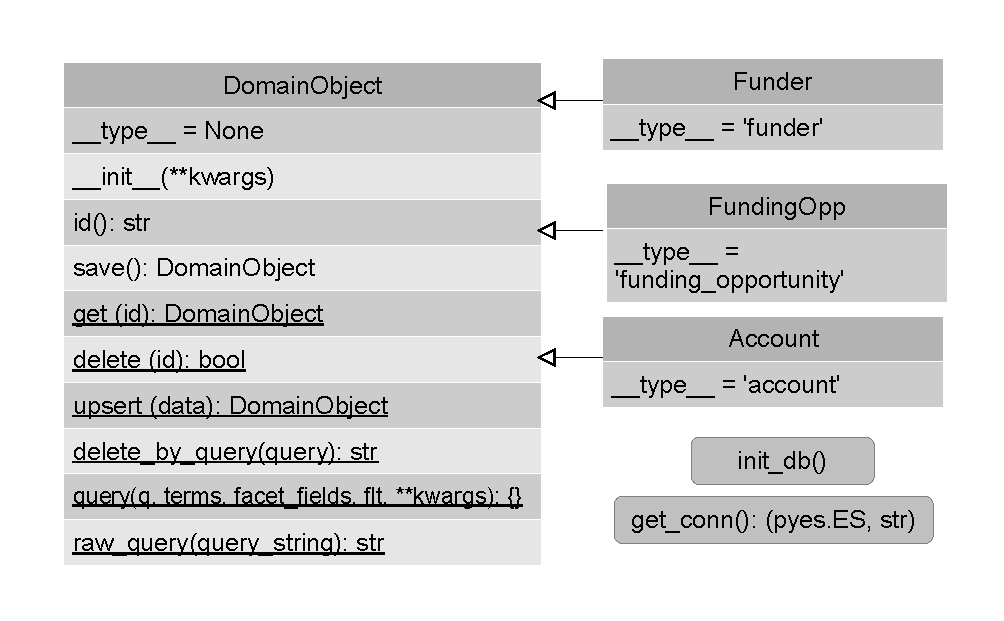
\includegraphics[width=1.00\textwidth,]{Chapter3/dao.pdf}
\caption{dao module overview - 3 classes and 2 functions}
\label{fig:dao}
\end{figure}

The |DomainObject| class defines all the necessary operations. Most of them are defined as class methods since instantiated DAO objects are rarely used in the codebase - since it's a web application, the in-memory objects are lost from one request to another, or one page to another. Instead, the datastore is used for persistence.

|DomainObject| inherits from |UserDict.IterableUserDict| in the core Python libraries, which means that it and its subclasses can be treated as a normal Python dictionary, and normal Python dictionaries can be easily converted into these classes. In practice, this means being able to do things like |funder['name'] = request.values.funder_name| as well as being able to create objects by doing:

\begin{verbatim}
incoming_data_dict = {
    'name': request.values.funder_name,
    'tags': process_the_tags_function(request.values.tags),
[...]
}

[...]

new_funder = dao.Funder(incoming_data_dict)
\end{verbatim}

Everything in the datastore is a dictionary (or a list) so the objects themselves serve no further purpose that to define the type of the document which is being uploaded. Thus the |upsert| static method, which takes care of uploading documents to the index, takes a simple dictionary and uploads its contents to the datastore. The only difference between a user |Account|, a |Funder| and a |FundingOpp| is in the class name and associated |__type__| value, which gets passed on as the first argument to |upsert| in this line:

\begin{verbatim}
new_funder = dao.Funder(incoming_data_dict) # note class name
    # telling upsert what type the document is
\end{verbatim}

The |upsert| method also generates and includes |id|s in incoming data, unless the data already contains an id. This gets executed for all objects which are uploaded to the index, making it easy to change the |id|-generating algorithm. It can also be overridden on a per-class basis, i.e. |Account| may wish to generate different |id|s if they are not specified.

The |get| and |delete| static methods take an object id and operate on it (either getting the contents from the datastore or deleting that document).

|delete_by_query|, |query| and |raw_query| simply provide means of interacting directly with the datastore to fetch or delete a larger group of documents.
% Datastore section below says It's done in a fairly elegant, generic way, described in \myref{design-dao}.

\subsection{web}
\label{design-web}
This module is the ``web server'' of the application – it defines the routes and the corresponding functions which handle them (in a RESTful way), runs constantly and outputs exceptions to standard output. If more logic is needed to respond to a certain request than will fit comfortably in one short function, then the function can load another module (e.g. Importer).

If the HTTP POST and GET processing differ a lot, or other advanced features are needed, then Flask ``views'' can be used - these are classes which respond to HTTP requests.

The two ways to do routing in Flask which FundFind uses are illustrated below.

This is the route to the index, or home page. It does nothing but call on the Flask framework to process the given template (which is in Jinja2 format, not pure HTML as the extension suggests) and serve it to the user.
\begin{verbatim}
@app.route('/')
def home():
    return render_template('home/index.html')
\end{verbatim}

This is a slightly more elaborate example:
\begin{verbatim}
class ShareFundoppView(MethodView):
    '''Submit information about a funding opportunity'''
    def get(self):
    # respond to HTTP GET
        if current_user.is_anonymous():
	[...] # do some processing
        return render_template('share_fundopp.html',
	  active_page='share_fundopp')

    def post(self):
    # respond to HTTP POST
        if current_user.is_anonymous():
            abort(401)

	    [...] # do some data validation
            return render_template('share_fundopp.html')

# Register the view
app.add_url_rule('/share_fundopp', 
  view_func=ShareFundoppView.as_view('share_fundopp'))
\end{verbatim}

The last line adds the new view class to the routes, so that it will be handed all requests which come in at |/share_fundopp|.

|web| also defines a few functions to help with logging users in - more details in \myref{impl-create-profiles}.

These are all routes that |web| defines:
\begin{itemize}
\item GET |/| - home page
\item GET |/account/<user>| - view a user profile
\item GET |/content/<path:path>| - generic route to server ``static'' content like tutorial pages, API pages and so on (only works if the supplied filename actually matches a template, otherwise 404 Not Found)
\item GET, POST |/search| - search for funding opportunities and funders
\item GET, POST |/describe_funder| - share information about a funding organisation
\item GET, POST |/share_fundopp| - share information abotu a funding opportunity
\item GET, POST |/slugify| - exposes the |util.slugify| function to the world via the API. This is mainly of use for AJAX requests, which are briefly discussed in \myref{design-ajax}, although API consumers could use it if they wish to.
\end{itemize}


\subsection{importer}
\label{design-importer}
A module which contains the Importer class. This handles data collection – submissions to FundFind via the |/describe_funder| and |/share_fundopp| routes. The Importer class gets instantiated and used by the |web| module. This is a pretty simple module which mostly deals with processing the data coming in from the API or the user interface information sharing forms. It has two methods - |describe_funder| and |share_fundopp| which mostly clean up incoming data. The data is retrieved from the |request| object, which is a Flask framework-provided object which represents the current HTTP request - all its parameters (in |request.values|) and other related information.

The module does define three internal helper methods, which could arguably be moved to the |util| module if there was any use for them anywhere else in the codebase:
\begin{enumerate}
 \item |_clean_list| takes a list of items and strips whitespace off both ends of each item in the list. For example, if ['tag1', ' tag2', 'tag3 '] come in, it will return ['tag1', 'tag2', 'tag3']. This can happen quite easily since users are allowed to enter tags as a comma-separated string on the user interface, and this is then broken up by removing the commas and putting the resulting parts in a list - but it doesn't handle whitespace.
 \item |_prep_link| takes a string representing a URL (e.g |'www.aber.ac.uk'| and prefixes it with |'http://'| if it doesn't already start with |'http://'| or |'https://'|.
 \item |_str2isodt| converts incoming strings to Python datetime values. It uses the third-party |parsedatetime| module to try and guess the date format, since this module supports more formats than a single person can (usually) imagine.
\end{enumerate}


\subsection{config}
This class is a wrapper around a simple JSON dictionary of key-value pairs which contains hard-coded configuration information.

The root directory of the repository contains |config.json|, which looks like:
\begin{verbatim}
{
    # service
    "service_name" : "FundFind",
    [...] # more settings
}
\end{verbatim}

The |config| module makes it possible to say |from fundfind import config| in, for example, the |dao| module. The wrapper functionality essentially allows |config['service_name']| to then return |"FundFind"|, going by the example above.

\subsubsection{default\_settings}
|default_settings| is a Python file which simply contains several constants that toggle various user interface frameworks' options, like:

\begin{verbatim}
# override certain defaults of the Flask-Bootstrap extension
BOOTSTRAP_USE_MINIFIED = False # small performance gain not worth loss of debugging info yet
BOOTSTRAP_JQUERY_VERSION = '1.9.1' # most up-to-date that's tested with the app
\end{verbatim}

The information is merged with the rest of the configuration when it is loaded.

The reason there are two separate modules is because this design was recommended - this is a fully-featured Python file which could do far more than simply stating values, like the |config.json| file has to. The reason the |config.json| file still exists is that it works, it is easy to understand and work with, and it simply has not yet been merged into |default_settings|. It is debatable whether the configuration should be kept in a code module or more a immediately visible location such as the root of the code repository. Time constraints preclude such debate in this project, however.

\subsection{util}
Currently defines just one function.

|slugify| turns normal text (including Unicode text) into a more restricted version of URL-friendly text, called a ``slug''. It replaces whitespace and other delimiters and punctuation with underscores. For example, ``Inertial Fusion Energy  in the UK and Beyond       -  !?'' becomes ``inertial\_fusion\_energy\_in\_the\_uk\_and\_beyond''.

% \subsection{suggest}
% The |suggest| package serves as a facade - if |import suggest| is specified, it bundles together functions from the underlying modules to expose functionality like |from suggest import projects| or |from suggest import funding_opportunities|. In other words, the caller does not have to know the implementation details - they do not have to care about the fact that |gtr| and |hypothethical_module1|suggest projects, but |hypothethical_module2| suggests funding opportunities. Not having to know the names also helps easily maintain backwards compatability - if, for some reason, the |gtr| module is renamed to |gateway_to_research|, it will not break all the code which is importing the |suggest| package.
% 
% At the moment it \emph{only} contains the |gtr| module, which can only suggest projects, so only |from suggest import projects| will work.
% 
% \subsubsection{gtr}
% Contains the |GTRConsumer| class which communicates with the Gateway to Research API. Its |suggest| method returns a list of the items which Gateway to Research returns given the user's query to FundFind. The query is just passed on to GtR and the results are displayed on the user interface without further processing.

\section{fundingharvest}
\label{design-main-last}

\subsection{base}
\label{design-fundingharvest-base}
This module contains the |BaseHarvester| class which contains no functionality, but is there in case child classes need common functionality which happens to have the same implementation. Utility functions such as |check_results()| (ensure results being returned to the code have certain keys) are one example.

This is presently less useful in its current form since there is only one class which inherits from it - |RSSHarvester|. However, the initial design for the Funding Harvest project including a |CLISubmitter| which ``harvested'' information from the command line (i.e. tested the whole idea).

It also used to include an |EmailHarvesterBase| which was meant to provide common functionality for trying to parse e-mails, like connecting to an IMAP server and fetching the right e-mail (last in reverse chronological order to match a certain subject line and possibly other header conditions). |EpsrcEmailHarvester| would then connect to it. The feature was unfortunately dropped since it turned out to be too difficult to implement in the remaining time/priority considerations (see \myref{impl-email-parse}). However, |fundfind.email.harvester@gmail.com| has been created and is receiving weekly alerts from the EPSRC.

Therefore, the inheritance structure has been kept, keeping \myref{future-work} in mind.

\subsection{rss}
This module contains the |RSSHarvester| class which aims to provide common functionality such as |load_rss_feed()| to its children.

\subsection{rcuk\_esrc}
\label{design-rcuk-esrc}
This module contains the |EsrcRssHarvester| class which consumes the RSS feed of the ESRC (Economic and Social Research Council). This council was chosen since their RSS feed \cite{esrc-rss} actually takes arguments such as search terms and time periods. RSS feeds are not supposed to be used like that - they ought to only contain the latest items since a server-determined date, usually a week or so. This is a really interesting case of somebody using their RSS publishing capabilities as an ad-hoc API, even allowing users to do what is essentially search queries, but not having to code an API or a user interface on top - just relying on the user to input the URL they want and bookmark it in their RSS reader!

However, this detail also made this feed very easy to use for a prototype project such as FundFind - Funding Harvest would have had to be subscribed to other organisations' feeds for several weeks to get a good amount of useful data into the datastore.

\section{User Interface}

The user interface is pretty simple - two information submission forms and a search page (which doubles up as a ``view records'' page) as well as a ``my account'' page.
%TODO screenshots here

Designing a user interface usually revolves around two questions - what is being exposed (data, functionality) and how it is being exposed so that it can be best utilised by the users.

\subsection{Content}
The content or ``what'' to display was driven almost solely by what values the data had in general. Examples taken into account were EPSRC \cite{epsrc-example} and Wellcome Trust \cite{wellcome-example} pages and the RSS feeds of BBSRC {bbsrc-rss} and ESRC {esrc-rss}.

The process went as follows:
\begin{enumerate}
\item look at available data from the listed sources
\item change the funding opportunity submission page, adding newly observed fields
\item later on, look through the data and see what the search/view page is unable to show and enhance its knowledge of the data
\end{enumerate}

\subsection{Exposing the content}
\label{design-ui-exposing-the-content}
Web user interface libraries package a lot of professional UX (User eXperience) designers' and developers' knowledge into an easy to reuse package. Bootstrap \cite{bootstrap} is one such library and it was used together with jQuery \cite{jquery} and jQuery UI\cite{jquery-ui} to make FundFind's user interface, including the responsive mobile UI characteristic.

These libraries package their UX knowledge into individual components which can be mixed together in a user interface. Those components still have to be brought together by the developer in a web page, however.

The fields in the information submission forms were just ordered in order of perceived importance, mostly as presented in the data sources mentioned above. Fields related to FundFind were placed at the bottom (e.g. tags) since the best way to write such metadata is to have thought about the values in the rest of the form.

\subsubsection{Faceted Search}
\label{faceted-search}
Faceted search \cite{faceted} was chosen as a core concept to build the user interface on due to its ability to allow easy exploration of large semistructured datasets and quick drill-down to data the user is interested in.

At first, both the HTML user interface and the API were going to use this concept. However, faceted search is actually good for semistructured data because human minds are good at processing it. That is, as long as the data is analysed on the fly and  common fields and values are presented, as well as basic frequency analysis (how many times does value Y appear in field X). At the Gateway to Research hackday it became obvious quite quickly that the developers present did not care that much for the ``didYouMean'' key in the results as much as the raw data - and the raw data could only be retrieved through a pagination mechanism. Thus, the otherwise nice feature which helps human users a lot was not used at all as developers tried to page through the GtR API to retrieve a wholesome dataset from it - a question of different priorities. That is why the idea of including facets in the API has been dropped for the moment, as it is best to start from what API clients would actually want - the most basic being just the data - and then trying to find what further features they might want.

``Facets'' can be thought of as the various ``columns'' of a dataset if it was flattened out into a CSV file or a SQL database table. Each record in the dataset has a some value in each column, and blanks are allowed. The analysis / aggregation of the unique values in a column is called a ``facet''. A (simplified) example of what the data for this project might look like can be seen in Table \ref{tab:facets-example}.

\begin{table}[!h]
\centering
\begin{tabular}{p{8cm}|l|l|r}
	Opportunity name & Subject & Country & Funder\\
	\hline
	Shadow manipulation in automatic understanding of 3D representations of real-world video footage & Computer Science & UK & EPSRC\\[6pt]
	Say hello! A global qualitative study of greeting phrases & Psychology & USA & APA\\[6pt]
	Fast-Fourier and the Three Musketeers & Computer Science & UK & BBC\\
\end{tabular}
\caption{Example dataset for the purpose of illustrating what facets are}
\label{tab:facets-example}
\end{table}

If we choose to construct facets from the Subject and Country fields, they would look like the ones illustrated by Table \ref{tab:facets-example2}.
\begin{table}[!h]
\centering
\begin{tabular}{l|l|l}
	Facet name & Value & Number of items\\
	\hline
	Subject & Computer Science & 2\\[3pt]
	 & Psychology & 1\\[3pt]
	Country & UK & 2\\[3pt]
	 & USA & 1\\[3pt]
\end{tabular}
\caption{Example facets}
\label{tab:facets-example2}
\end{table}

Faceted search is often used for semi-structured data when producing an exhaustive classification is difficult since the data available in different records varies and there are many ways to classify it. One example is library catalogues like the ExLibris Primo software \cite{primo}, where the artefacts the user could be looking for vary from journal articles through manuscripts to books, span various fields and are grouped by subject - very much like funding opportunities can be.

%TODO examples here - from fundfind, even from other projects

\section{API}
\label{design-api}
  % divide into ``usability design'' - how usable API is by developers, what thought was put into that
  % and technical design
%   \subsection{Design for Developers}
%     % general waffle
%     The routes which would be of most interest to other software trying to communicate with FundFind are |share_fundopp|, |describe_funder|, |search| and |suggest|.
%     
%     For example, the developers of a hypothetical ``News for Scholars'' newsfeed reader application might want to suggest previously funded bids to its UK readers. They have two options:
%     
%     \begin{enumerate}
%      \item Re-use the classes within the Suggest module which enable FundFind's ``this may be of interest'' feature. If the hypothetical application is written in Python, this will just involve copying $+$ editing the code and perhaps reading the Gateway to Research API documentation (for the UK information). If it is written in another language, ``re-use'' will mean looking at the logic contained within the |suggest| package and re-implementing it, both of which are relatively time-consuming.
%      \item The other option is to send a request to FundFind's |/suggest| route and use the results.
%     \end{enumerate}
%     
%     While \#2 needs to be used with great care in production environments (\#1 is clearly preferable to FundFind maintainers due to resource usage in this case), it can certainly be used to get a feeling for what the results can be, or in a development version of the application.

The API was implemented by using Flask's capabilities to declare handling of HTTP GET and POST in an easy way, described in \myref{design-web} and by detecting whether the request wants JSON format. If not, the HTML user interface is served.

\subsection{Data format}
  JSON was used as the API's main data format mainly due to interoperability reasons - it is extremely simple and as such has support in most major programming languages. Furthermore, if it assumed that other Open Knowledge-related projects are most likely to use FundFind's API, then the fact that a lot of them are written in Python (as mentioned in \myref{design-rationale}) plays a role. Python has excellent support for JSON through a core library and more importantly, its most popular internal datastructures - dictionaries and lists - resemble JSON perfectly, making it easier to read and ``digest'' for Python programmers.
  
  Furthermore, FundFind uses JSON itself when communicating with its elasticsearch datastore, again via an API, and there was not much reason to introduce another transport medium at this stage of a prototype project.
 
%\section{Alternative Designs}